Knowing the problem exposed in the previous section, the "ideal" surface over which the power is calculated has to be estimated. Then the influence of the geometrical parameters on the performances (estimated by the condition number of the \gls{V2PM}) can be studied. 

In all the following, the amplitude of visibility (or visibility) refers to $V_{ij}$ (sometimes to the all function $V_{ij}cos(\phi_{ij})$ where $\phi_{ij}$ is a function of the \gls{opd}. A good approximation of $\phi_{ij}$ is $\frac{2\pi x}{\lambda}$ where x is the \gls{opd}. $V$ and $\phi$ are both obtained by fitting the simulated curve with a cosine.


To estimate the critical surface, the power at an output versus the \gls{opd} is simulated using the software $BeamProp^{TM}$. It has been found that the presence of harmonics in the signal should not be higher than 2\% of the main signal (the cosine). A surface corresponding to the waveguide's cross-section appeared to solve this problem for a wavelength of 3.8\si{\micro\meter} as shown on Fig.\ref{fig:harmonics}.   


\begin{figure}[htbp]
  \centering
  \begin{minipage}[b]{.45\textwidth}
    \centering
    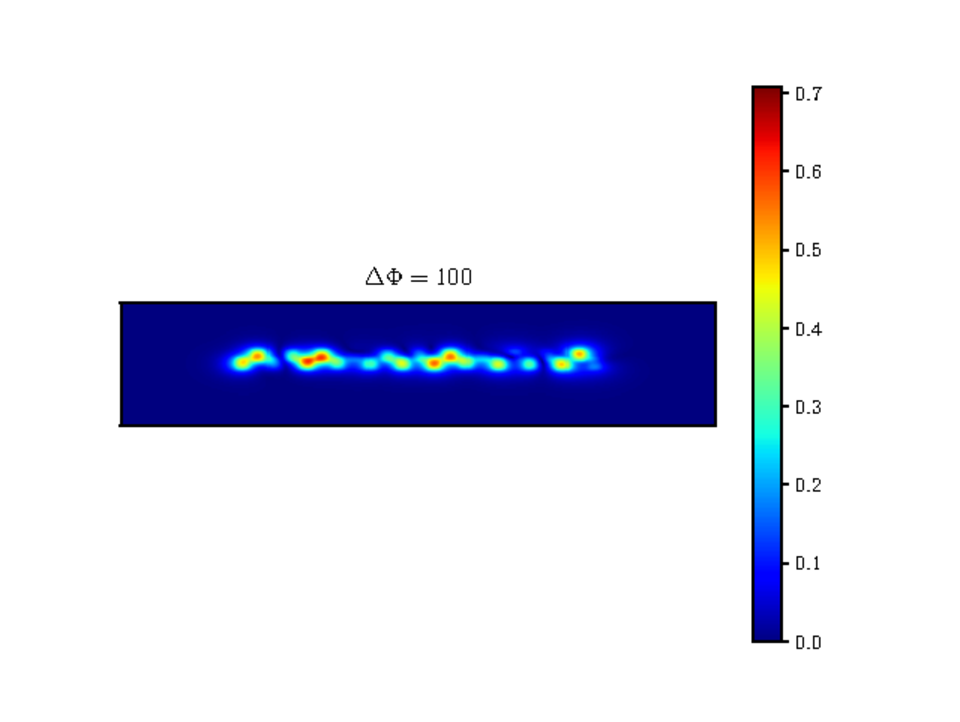
\includegraphics[scale=.5]{../picture/phase_100.pdf}
    \subcaption{Example of the output simulated field.}
    \label{fig:notcentered}
  \end{minipage}%
  \hspace{0.5 cm}
  \begin{minipage}[b]{.45\textwidth}
    \centering
    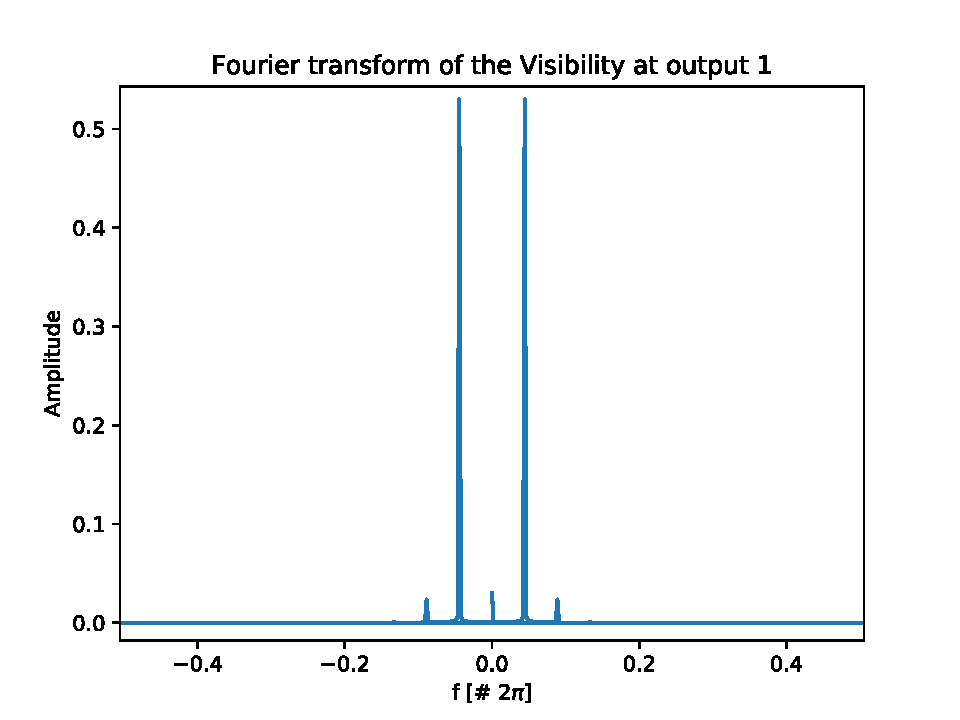
\includegraphics[scale=.5]{../picture/Fourier_1.pdf}
    \subcaption{Spectrum of the visibility at output 1}
    \label{fig:harmonics}
  \end{minipage}
  \caption{Origin and presence of harmonics in the output calculated
    power}
\end{figure}

All simulation unless explicitly written are performed using the previously determined integrating area. Moreover the base parameters : $P_x=24\si{\micro\meter}$, $P_y=10.8\si{\micro\meter}$,
$width=9.5\si{\micro\meter}$, $height=17\si{\micro\meter}$, $\delta n
= 0.005$, $\lambda=3.4\si{\micro\meter}$, length of the DBC's part $= 25mm$, length of the input $=25mm$, together with transparent boundary
condition. The grid dimensions and z step are chosen as a balance between computation time and desired accuracy. For general results one can
choose a <<coarse>> grid and then narrow it for more accurate results.
Results presented are for scalar solution of the wave equation. Therefore
they do not incorporate impacts of polarization effects. Moreover the material are supposedly
perfects in the simulation (i.e. isotropic material, no absorption, no scattering...).


To ensure a good accuracy on the retrieved astronomical parameters,
the V2PM's condition number must be as close to 1 as possible (see
\ref{an:cond}). This part will be focused on lowering the V2PM's
condition number by using different geometrical parameters. 
The launch fields are Gaussian of same power and of 1/e diameters the
width and height of the wave-guide. Thus a coupling loss of
approximately 10\% occurs. Fresnel losses are not included.

\paragraph{X and Y spacing:}
Simulations were performed for different values of $P_x$ and $P_y$ to
find which parameters minimizes the condition number. The results are
shown in table \ref{tbl:cond_vs_pxpy}. With the few tested parameters
one can only conclude that the V2PM condition number seems to be minimum for $P_x \approx 24 \si{\micro\meter}$ and $P_y \approx
10.8 \si{\micro\meter}$. Concerning the throughput, it seems to have a
quite linear dependency with $P_y$ and an exponential decay with $P_x$ within the tested
range (and only within the tested range as the throughput should stay between 0\% and 100\%). Fitted results are displayed in figure
\ref{fig:throu_pxpy}. Theses results are obtained for one set of
parameters and should be valid only within the tested range.

\begin{table}[htbp!]
\centering
\begin{tabular}{|>{\begin{bf} \columncolor{gray!20}} c <{\end{bf}}|c|c|c|c|c|}
\hline
\rowcolor{gray!20} \diagbox{Px[$\mu m$]}{Py [$\mu m$]}&\bf{4.8} &\bf{6.8}  & \bf{8.8}            & \bf{10.8}           & \bf{12.8}          \\ \hline
19          & &         &                & 10.68 (67.1\%) &
                \\ \hline
21          & &         &                & 10.69 (63.1\%) &               \\ \hline
23          & &         &                & 24.77 (61.5\%) &               \\ \hline
24          &24.05 (62.3\%) &   32.6 (62.0\%)      & 18.77 (61.7\%) & 7.16 (61.2\%)  & 16.6 (60.8\%) \\ \hline
25          & &         &                & 11.7 (60.9\%)  &               \\ \hline
\end{tabular}
\caption{Condition number and throughput (in parenthesis) for several x and y spacing. The throughput is calculated by the sum of the
  power at each outputs normalized by the total input power. The power is calculated by a power integral of the simulated field over the wave-guide's cross-section}
\label{tbl:cond_vs_pxpy}
\end{table}

\begin{figure}[htbp]
  \centering
  \begin{subfigure}[b]{.45\textwidth}
    \centering
    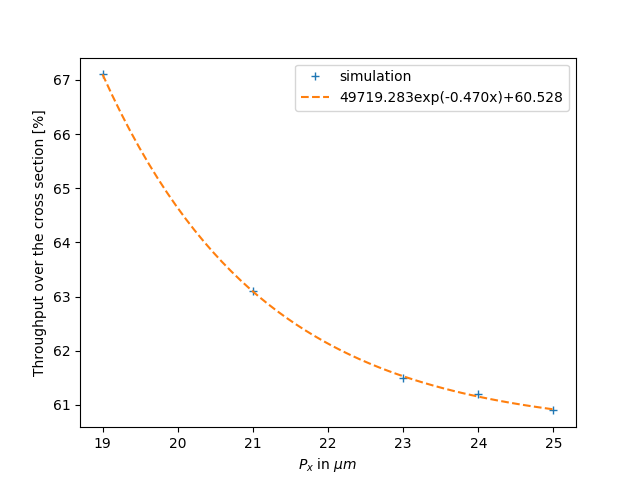
\includegraphics[scale=.4]{picture/geometry/throughput_px.png}
    \subcaption{}
  \end{subfigure}%
  \hspace{.5cm}
  \begin{subfigure}[b]{.45\textwidth}
    \centering
    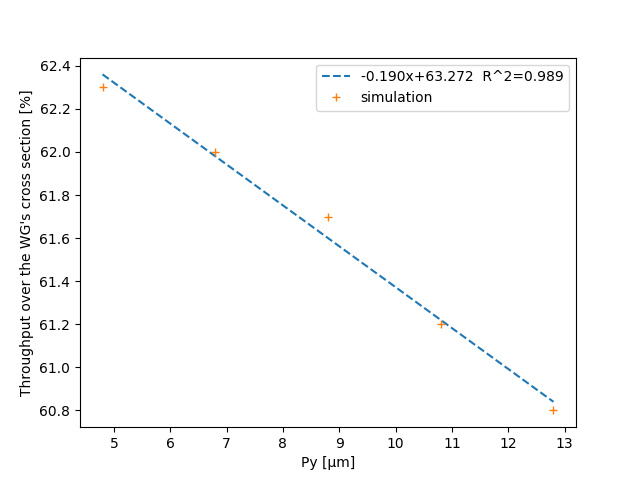
\includegraphics[scale=.4]{picture/geometry/throughput_py.png}
    \subcaption{}
  \end{subfigure}
  \caption{Evolution of the throughput over the cross section with
    $P_x$ and $P_y$ at fixed cross-section and simulation
    parameters (see text for details). (a) at fixed $P_y=10.8 \mu m$, (b) at fixed $P_x=24 \mu m$}
  \label{fig:throu_pxpy}
\end{figure}

\paragraph{The cross section:}
Now that a minimum of the condition number regarding x and y spacing
has been found, the wave-guide's dimensions has to be optimized
too. In the tested range all dimensions ensure that the wave-guide is
mono-mode to have all <<ray>> traveling at the same speed in z
direction (in the fundamental mode, most of the energy is traveling
close to the core of the WG). This is to ensure a low modal dispersion
and low coupling losses of the input field. These simulations are
performed for $P_x=24\si{\micro\meter}$ and
$P_y=10.8\si{\micro\meter}$.

\begin{table}[htbp!]
\centering
\begin{tabular}{|>{\begin{bf} \columncolor{gray!20}} c <{\end{bf}}|c|c|c|c|}
\hline
\rowcolor{gray!20} \diagbox{width}{height}& \bf{15} & \bf{16}            & \bf{17}
  & 18          \\ \hline
7.5 & & & 5.07 (45.9\%)& \\ \hline
8.5         &          &                & 8.00 (54.1\%) &               \\ \hline
9.5            &  7.76 (57.8\%)     & 8.29 (59.5\%)  & 7.16 (61.2\%) & 10.12 (62.4\%)         \\ \hline
10.5    &              &                & 14.6 (67.5\%) &               \\ \hline
\end{tabular}
\caption{Condition number and throughput (in parenthesis) over the WG's cross-section for several width and height. The throughput is calculated by the sum of the power at each outputs normalized by the total input power. The power is calculated by a power integral of the simulated field over the wave-guide's cross-section }
\label{tbl:cond_vs_wxwy}
\end{table}

One more time a minimum of the condition number is found for
$width=7.5\si{\micro\meter}$ and
$height=17\si{\micro\meter}$, but as such a width would lead to too much more refinance (which our simulation doesn't take into account) a width of $9.5 \si{\micro\meter}$ will be used instead. 
%\todo[inline]{Revoir la derniere phrase+plots ?}
The throughput seems to be linear for dimensions of the wave-guides slightly different. But only for dimensions closes to the simulated ones.

\paragraph{Optical index difference:}
The wave-guides used are rectangular dielectric wave-guides with step
index. As a higher optical index difference lead to a stronger mode
confinement, a higher throughput over the cross section is to be
expected with a higher $\delta n$. This paragraph focuses on finding
the best $\delta n$ to have an higher throughput together with a low
condition number of the V2PM matrix.
In this simulation the previously <<optimised>> geometrical parameters
are used (except for the width of the WGs which is $width=9.5\mu m$) and the throughput is still calculated over the wave-guide cross-section. The results are shown in table \ref{tab:cond_vs_delta_n}.

\begin{table}[htbp!]
\centering
\begin{tabular}{|>{\begin{bf} \columncolor{gray!20}} c <{\end{bf}}|c|c|}
\hline
\rowcolor{gray!20} $\delta n$ & condition number  & throughput  \\ \hline
0.002                   &     61.3           & 23\%    \\ \hline
0.003                 &13.5 & 40\%        \\ \hline
0.004                 & 6.1 & 52\%        \\ \hline
0.005                 & 7.16 & 61\%       \\ \hline
0.006                 & 15.0 & 68\%       \\ \hline
0.007                 & 14.6 & 73\%       \\ \hline
\end{tabular}
\caption{Condition number and throughput over the WG's cross-section
  for several values of $\delta n$. The throughput is calculated by the sum of the
  power at each outputs normalized by the total input power. The power is calculated by a power integral of the simulated field over the wave-guide's cross-section}
\label{tab:cond_vs_delta_n}
\end{table}

It seems that the throughput evolves as the logarithm of $\delta n$
within the tested range (and only within the tested range)(see fig.\ref{fig:throu_dn}).

\begin{figure}[htbp]
  \centering
  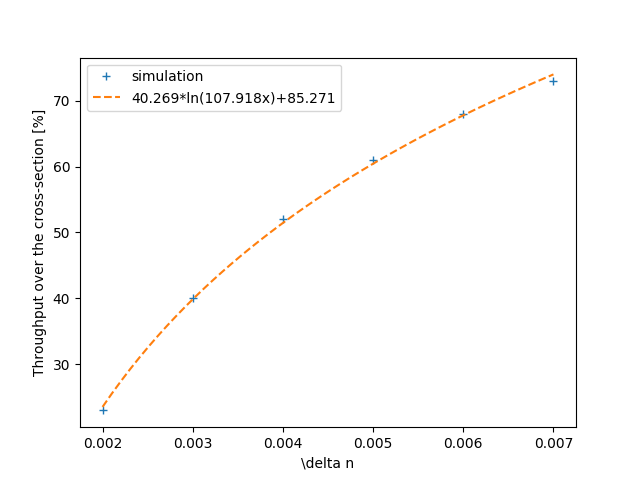
\includegraphics[scale=.5]{picture/geometry/throughput_dn.png}
  \caption{Throughput over the cross section for different optical
    index differences}
  \label{fig:throu_dn}
\end{figure}

The condition number seems to be minimum for $\delta_n=0.004$ but as it
is only of 1 lower than for $\delta_n=0.005$ and the throughput over
the wave-guide's cross-section is 10\% greater in this case, $\delta_n=0.005$ would be used as
<<optimised>> optical index difference.

\paragraph{Lengths:}
An other parameter that has to be optimized is the length of the
DBC's part. To this point all simulations were performed for a length
of $25\si{\milli\meter}$. An other length that could be optimized is
the length of the inputs which were also to this point of
$25\si{\milli\meter}$, but as the x and y spacing of the inputs ensures
that the fields aren't coupled, this shouldn't impact the V2PM
condition number. This was verified in the simulation for length
greater to $1cm$.
The results are shown in figure \ref{fig:length}. The <<1/e>> area
refers to a rectangle of width and height the 1/e width and height of
the fundamental mode of the wave-guide (for $\delta n=0.005$ which should contains 91\% of
the mode power)

The simulations were performed for a length greater than 15mm to be
sure that each inputs field propagates through the 23 outputs as can
be seen in the figure \ref{fig:propagation_L}.

\begin{figure}[htbp]
  \centering
  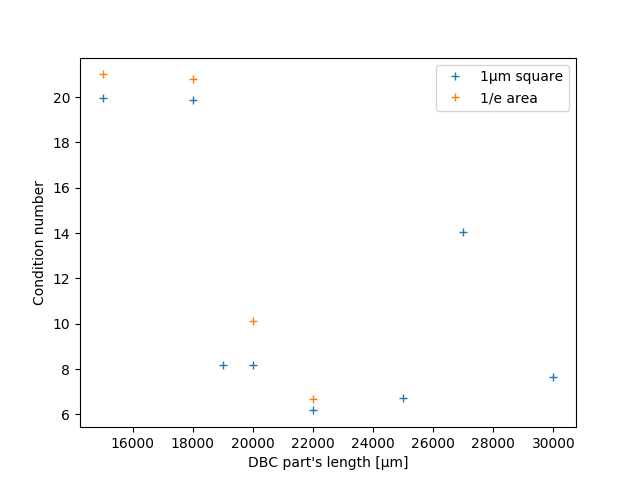
\includegraphics[scale=.5]{picture/geometry/CondNvsL.png}
  \caption{Condition number of the V2PM matrix for different lengths
    of the DBC part. The power is calculated either over a 1 by 1
    micrometer area or the <<1/e>> area centered on the
    cross-section. (see text for details)}
  \label{fig:length}
\end{figure}
One can notice that the condition number tend to be higher
for a short length of the DBC's part, and have a minimum of 6.15 for a
DBC part of 22mm
long. Moreover with a higher power integrating area, the condition number
seems to behave the same for a large or a small integrating area so
that a minimum of the condition number found with an integrating area
should remain a minimum for another (if the area isn't too large and
doesn't overlap surrounding fields).

Concerning the throughput, it seems to be constant within the tested
length (see Fig.\ref{fig:throughput_L}). Of course our simulated WG doesn't include scattering, surfaces defaults etc. The only kinds of losses that occurs
in this simulation are bending losses and
radiation in the cladding (absorption is negligible). The reader may have noticed a 10\% higher
throughput than in the previous sections. This is because the input
field in this simulation is a Gaussian of <<1/e>> width and height the
<<1/e>> width and height of the fundamental mode of the WG. Thus the
10\% coupling losses experienced in the previous do not take place in
this simulation.

\begin{figure}[htbp]
  \centering
  \begin{minipage}[b]{.45\textwidth}
    \centering
  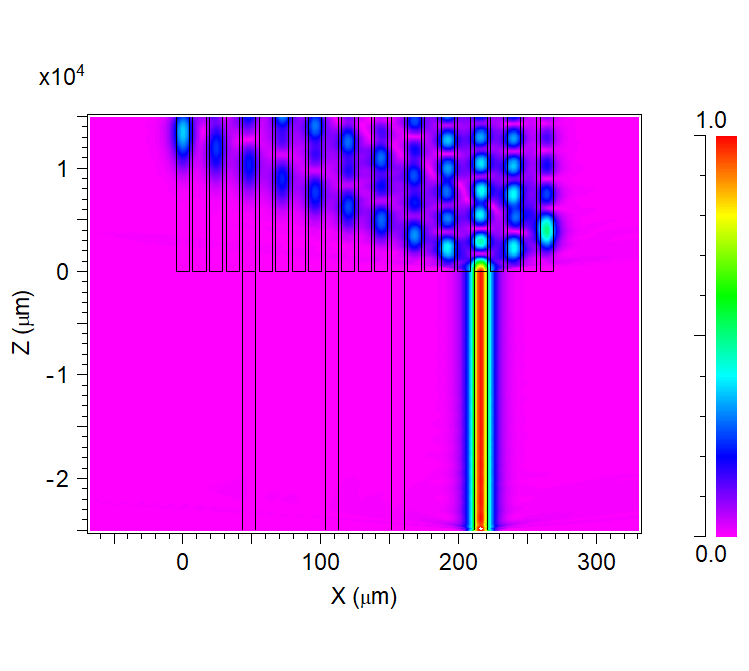
\includegraphics[scale=.25]{picture/geometry/propagation.png}
    \subcaption{Propagation of the scalar field from the 4th input. A
      length of 12mm seems to be a minimum to have the field reaching
      every single output.}
    \label{fig:propagation_L}
  \end{minipage}%
  \hspace{0.2 cm}
  \begin{minipage}[b]{.45\textwidth}
    \centering   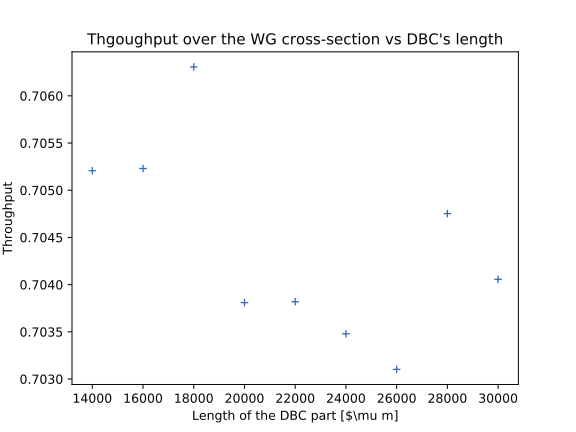
\includegraphics[scale=.35]{picture/geometry/throughput-L.png}
    \subcaption{Throughput over the cross-section for different
      lengths of the DBC part. Two area are considered to estimate the
    power at the outputs (see text for details).}
    \label{fig:throughput_L}
  \end{minipage}
  \caption{}
\end{figure}

It has be seen that the V2PM matrix is quite dependent of the area
over which the power is calculated at the output. One possible way to
minimise this dependency would be to design a <<fan-out>>. By
increasing the spacing of the outputs, the field should be more
centered and no overlapping would occur at the output. The next section
will focus on this component.

\subsubsection{Adding a <<fan out>>}
We have seen that both the visibility and phases relations are
dependent of the way the power is calculated. This is caused by the
fields overlapping at the outputs. One way to get rid of this effect
could be to add a <<fan out>> at the end of the DBC part and then be able to really take into account of all the flux when calculating the power. Simulations
with this have been performed with a spacing of the outputs of 2 times
the <<1/$e^3$>> width of the fundamental mode to be certain that no
more overlapping will occur (see Fig. \ref{fig:outputfield}). The length of the fan-out is chosen in order to limit bending loses and 1 cm appeared to be enough. A short straight section of 2 mm is added in order that all the flux have enough length to be well centered in the WG. By doing this one can estimate the
power in a wave-guide over a finite area and knowing which percentage
of the power of a Gaussian field is contained in the same area,
retrieve the total guided power (assuming that the fundamental mode is a Gaussien). But the point is that with such a
device, the way of calculating the power at the output should no more
impact neither the visibility nor phases relations, ergo the V2PM condition number (as it is the case with the previous component for large integrating area).
Therefore in these simulation the power is calculated by the power
integral of the simulated field over the WG's cross-section.
Results show that most of the visibility in that case are between
0.98 and 1.00 (without any polarization effects they should be all of
1) where they could be below 0.3 without the fan out.
Moreover with the simulated design the fan-out lead to less than 3\%
losses (bending losses and radiation in the cladding) as the
throughput over the WG's cross-section is up to 68\%.
A simulation of the throughput where the power at the end of each
output is calculated over a large enough area to consider that all the
power is being accounted we obtain 96.7\% of throughput. This results
could seems high but it is to be known that the simulations doesn't
take into account scattering, material absorption (which might be very
low for the considered material (GLS) at this wavelength) etc... Losses are only radiations in
the cladding, bending losses and coupling losses with the input field
(which we managed to get below 1\% in this simulation).
Moreover one can see that 68 is almost 71\% of 96.7 which is the
percentage of the true centered Gaussian field's power calculated over
the cross-section of the WG. This shows that at the outputs the fields
should be mostly Gaussian centered fields thus the <<fan out>> might be well designed.

\begin{figure}[htbp]
  \centering
  \begin{minipage}[b]{.45\textwidth}
    \centering
  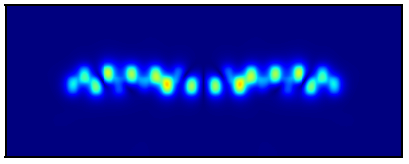
\includegraphics[scale=.5]{picture/geometry/phase_180_14.png}
    \subcaption{Output of the ZigZag DBC without fan-out. Fields are
      highly overlapping and not centred in the WG.}
  \end{minipage}%
  \hspace{0.2 cm}
  \begin{minipage}[b]{.45\textwidth}
    \centering   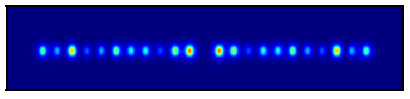
\includegraphics[scale=.5]{picture/geometry/phase_180_14_plat.png}
    \subcaption{Output of the ZigZag DBC with a <<flat>>
      fan-out. Fields are centered in the WG and not overlapping.}
  \end{minipage}
  \caption{Effect of adding a <<flat>> fan-out at the output. The
    color-scale is the same (0 in blue to 0.6 in red) and the scalar field is displayed.}
  \label{fig:outputfield}
\end{figure}

With this geometry of the <<fan out>>, the condition number of the
V2PM matrix seems to behave the same with the length of the DBC's part. The simulation leads to a condition number of 6.89 for a length
of 22mm (11.61 for a length of 20mm and 7.87 for a length of
19mm). Table \ref{tab:cond_3_area} show for 3 different length of the
DBC part and for three area considered to calculate the power, how
much the condition number is now <<independent>> of the considered
area.
\begin{table}[htbp]
  \centering
\begin{tabular}{
>{\columncolor[HTML]{C0C0C0}}l lll}
\diagbox{Area}{Length {[}mm{]}} & \cellcolor[HTML]{C0C0C0}18 & \cellcolor[HTML]{C0C0C0}20 & \cellcolor[HTML]{C0C0C0}22 \\
$1/e^3$                              & 7.77                       & 11.73                      & 6.89                       \\
Cross                                & 7.87                       & 11.61                      & 6.90                       \\
$3\mu m$                             & 7.92                       & 11.64                      & 6.89
\end{tabular}
  \caption{Condition number of the V2PM matrix for 3 different area used to
    calculate the power at the outputs. The <<$1/e^3$>> correspond to
    an area of $27\times 35\si{\micro\meter}$ (and contain more than
    99\% of the fundamental's power), the <<Cross>> is the wave-guide's cross section and the 3pixels to an area
    of $3\times 3\si{\micro\meter}$}
  \label{tab:cond_3_area}
\end{table}
It also
seems that the component with the <<fan out>> behave the same than the
component without it except that the way the power is calculated at
the output doesn't impact much more the V2PM
matrix, visibility and phases relations as can be seen on figure
\ref{fig:visi_phases_area}. Of course the visibilities are still
impacted but they still are greater than 95\% for the majority (and
greater than 0.75). In the case without the fan-out the visibilities
were down to 0.4 or less.
\begin{figure}[htbp]
  \centering
  \begin{subfigure}[b]{.45\textwidth}
    \centering
    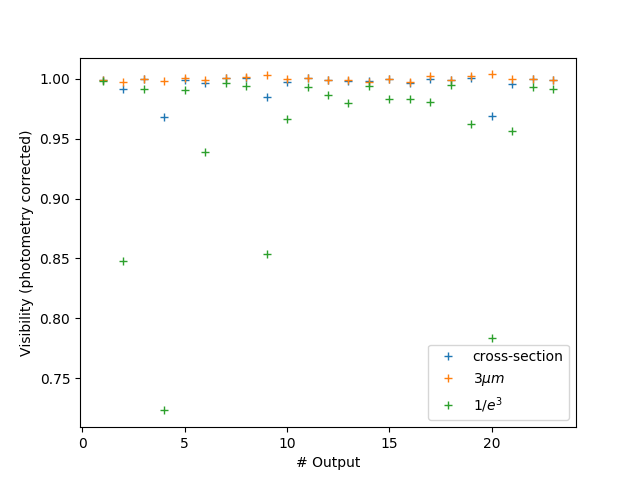
\includegraphics[scale=.4]{picture/geometry/visi_flat_3area.png}
    \caption{}
\end{subfigure}%
\hspace{.5cm}
\begin{subfigure}[b]{.45\textwidth}
  \centering
  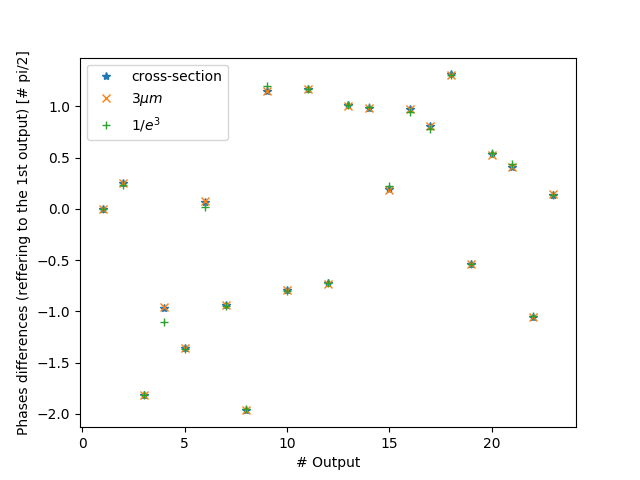
\includegraphics[scale=.4]{picture/geometry/phases_flat_3area.png}
  \caption{}
  \end{subfigure}
  \caption{Baseline 1-2 Visibilities (photometry corrected) and phases relations
    (referring to the first output) for 3 different area used to
    calculate the power at the outputs. The <<$1/e^3$>> correspond to
    an area of $27\times 35\si{\micro\meter}$, the <<1/e>> to an area of
    $15.596\times20.227\si{\micro\meter}$ and the 3pixels to an area
    of $3\times 3\si{\micro\meter}$}
  \label{fig:visi_phases_area}
 
\end{figure}

\paragraph{Effect of polarization on the retrieved parameters}
To this point no polarization effects has been simulated. In this part the V2PM matrix is calculated using monochromatic TE and TM polarized light. It is then studied the impact of using a TM polarization calibrated V2PM on the TE polarization data to retrieve the astronomical parameters (and vice et versa). 

First of all the V2PM calibrated matrix using TE polarized light show a condition number of 6.203 and it is  6.124 for the TM polarized light. In the case of the scalar field (no polarization effect) the condition number was 6.161 which is almost the mean of TE and TM ones. 
Those two V2PM matrices are used to retrieve the astronomical parameters from the simulated output fields. The results are shown in Tab.\ref{tab:retriev_polar} in which $\epsilon_i$ is calculated by $\epsilon_i=\sqrt{ \sum \frac{1}{N}(a-\tilde{a})^2}$  where $a$ is the data, $\tilde{a}$ the expected parameter (phase or visibility) and N the number of simulated phase and visibility.  One can see that the error on the retrieved parameters are between 30 and 40 times higher when using the V2PM calibrated using polarized light on 90° shifted polarized light.  The impact is still very low and justify not taking into account the polarization for the previous simulation.

\begin{table}[]
\begin{tabular}{|c|c|c|c|c|}\hline
\multirow{2}{*}{\diagbox[]{data}{V2PM}} & \multicolumn{2}{c|}{TE}                          & \multicolumn{2}{c|}{TM}                          \\
\cline{2-5}                  & $\epsilon_{\phi}$ {[}rad{]} & $\epsilon_V [\%]$ & $\epsilon_{\phi}$ {[}rad{]} & $\epsilon_V [\%]$ \\
\hline
TE                & $\num{0.000695}$            & $\num{0.000714}$  & $\num{0.0217}$              & $\num{0.0251}$    \\
\hline
TM                & $\num{0.0208}$              & $\num{0.0247}$    & $\num{0.000636}$            & $\num{0.000677}$
\\ \hline
\end{tabular}
\caption{Error on the retrieved parameters from the V2PM calibrated using TE/TM polarized light. The TE/TM data refers as the simulated input fields.}
\label{tab:retriev_polar}
\end{table}

\paragraph{adaptability to other wavelength}
Before simulating the \gls{dbc} using poly-chromatic light the dependence of the design regarding the wavelength is tested. Of course to have a component that behave the same at an other wavelength one can simply multiply its dimensions by the ratio of the wavelength. But as a component will have to be used using poly-chromatic light it is interesting to see how the condition number is influenced for a given design by the wavelength. The design previously "optimized" is used for this simulation. The results of this simulation are shown in Fig.\ref{fig:cond_mono_multi}. As can be seen both of the curves are very similar in first sight. The component without fan-out show a flat curve for lambda ranging from 3.35 to 3.43 $\si{\micro\meter}$ where for the component with fan-out this "flat zone" almost doesn't exist. This suggest that the component without fan-out could be more stable than the component with. This can be explained by the fact that the geometry of the fan-out act like if the coupling length were longer. This apparent length is strongly dependent of the wavelength because the coupling of the fields between two nearby waveguides are strongly dependents of the wavelength. The zone where the WGs separates will couple a larger wavelength for a longer length because of the larger overlap integral between the two  individual WG's modes for higher wavelength. For further explanation on the coupled mode theory the reader can refers to \cite{saleh_teich, marcuse}.


\begin{figure}
    \centering
    \begin{subfigure}{.45\textwidth}
        \centering
        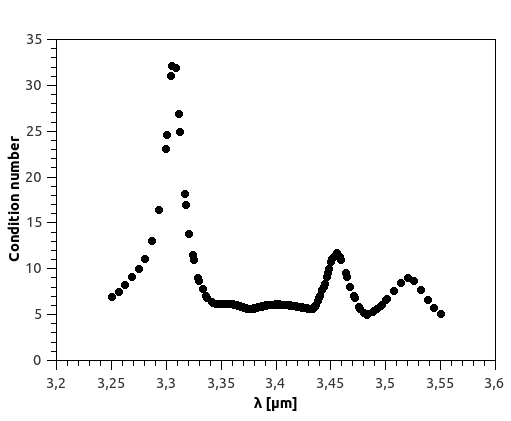
\includegraphics[scale=.45]{picture/cond_BW/nofan.png}
        \subcaption{}
    \end{subfigure}%
    \hspace{.5cm}
    \begin{subfigure}{.45\textwidth}
        \centering
        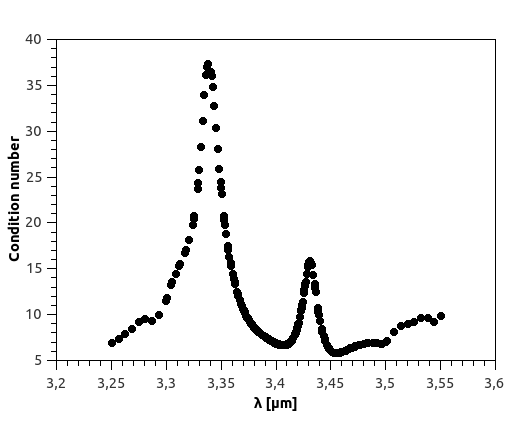
\includegraphics[scale=.45]{picture/cond_BW/fanout.png}
        \subcaption{}
    \end{subfigure}
    \caption{Condition number of monochromatic V2PM matrices at different wavelength. (a) for the component without fan-out, (b) for the component with fan-out. The geometry of the component is the optimized one (see text for details)}
    \label{fig:cond_mono_multi}
\end{figure}



The evolution of the V2PM's condition number regarding the geometrical parameters and the wavelength has been studied and an optimal configuration has been found. This configuration ensures a condition number of approximately 6 which means that an error on the measured output wouldn't be magnified more than 6 times (in the worst case) by the retrieving algorithm. The evolution of the "usable" throughput through a defined surface has also been studied and result of more than 96\% in the case of the component with fan-out and 70\% without. This throughput doesn't include the losses from coupling nor Fresnel which should be predominant for this component. The optimized parameters are given in Tab.\ref{tab:optimised_parameters}. All the previous work has been done using only monochromatic light. But the light from a star is obviously not monochromatic, an it's not wanted to use too narrow-band filters in order to keep high \gls{snr}. This is the purpose of the next section.


\begin{table}[htbp]
\begin{center}
\begin{tabular}{|c|c|}
%\cline{2-2}
\multicolumn{1}{c}{} &\multicolumn{1}{c}{} \\ \cline{1-2}
  $P_x$ & $\num{24}$ \\ \cline{1-2}
  $P_y$ & $\num{10,8}$\\\cline{1-2}
  $width$ & $\num{9,5}$ \\\cline{1-2}
  $height$ & $\num{17}$  \\\cline{1-2}
  $\delta$ & $\num{0,005}$  \\\cline{1-2}
  $\lambda$ & $\num{3,4}$ \\\cline{1-2}
  $L_c$ & $\num{22000}$  \\\cline{1-2}
  $L_i$ & $\num{10000}$  \\\cline{1-2}
  background index & $\num{2,31}$  \\\cline{1-2}
\end{tabular}\\
\end{center}
\caption{Optimised set of parameters (distance unit in \si{\micro\meter})}
\label{tab:optimised_parameters}
\end{table}
